\documentclass[reqno]{amsart}
\setlength{\parindent}{0pt}
\newcommand{\JMA}{\text{JMA}}
\usepackage{graphicx}
\title{Simulated TGA curves}
\author{Duncan and Rahul}
\begin{document}
\maketitle

We modify the simple Arrhenius pyrolysis model from Morvan and Dupuy 2001 (Combustion and Flame) for TGA curves to include the $\JMA(x,4)$ (called the fourth-order $\JMA$) reaction model for pyrolysis. 
The system of ODEs is 
\begin{align}
\frac{d}{dT} \alpha_s \rho_s Y_{H2O} &=\frac{1}{dT/dt}\frac{k_{H2O}}{\sqrt{T_s}} \alpha_s\rho_s Y_{H2O} \exp(-E_{H2O}/(RT_s)) \,,\\
\frac{d}{dT} \alpha_s \rho_s Y_{i} &=\frac{1}{dT/dt}k_{pyr}\alpha_s\rho_s Y_i \JMA(M/M_0,4) \exp(-E_{pyr}/(RT_s)) \,,\\
\frac{d}{dT} M_{O_2} &=\frac{1}{dT/dt}k_{char} M_{O_2} \exp(-E_{char}/(RT_s))\alpha_s \sigma_s \,,\\
%          -(1/dTdt)*kchar*y(3)*exp(-erchar./t)*y(4)*sigs./y(5);...
\frac{d}{dT} \alpha_s &=\frac{1}{dT/dt}\frac{k_{char}}{\rho_s}\alpha_s \exp(-E_{char}/(RT_s)) \,,\\
\frac{d}{dT} \rho_s &=\frac{1}{dT/dt}\big((\nu_{char}-\nu_{soot}-1) k_{pyr} \alpha_s \rho_s Y_i \nonumber \\ &\times \JMA(M/M_0,4) \exp(-E_{pyr}/(RT_s)) \nonumber \\
                    & -\frac{k_{H2O}}{\sqrt{T_s}} \alpha_s\rho_s Y_{H2O} \exp(-E_{H2O}/(RT_s))\big) \,,\\
\frac{d}{dT} \alpha_s \rho_s Y_{char} &=\frac{1}{dT/dt}\big( (\nu_{char}-\nu_{soot}) k_{pyr}\alpha_s\rho_s Y_i \nonumber \\ &\times \JMA(M/M_0,4) \exp(-E_{pyr}/(RT_s)) \nonumber \\
&-(\nu_{ash}/\nu_{char}+1) k_{char} M_{O_2} \exp(-E_{char}/(RT_s))\alpha_s \sigma_s \,.
\label{eqn:TGAmodel}
\end{align}

Notice that quantities like $\alpha\rho Y$ are masses of particular species. 
Once we have solved the system of equations, we can compute the individual mass fractions and we can reconstruct the mass loss curve by looking at mass as a function of solid temperature $T_s$. 
In TGA the heating rate is constant and the atmosphere is initially inert.

The $\JMA(x,4)$ model is defined as 
\begin{equation}
   \JMA(x,4)=4(1-x)(-\log(1-x))^{3/4}\,,
\end{equation} 
where $\log$ is the natural logarithm.
Because of the singularity in the $\JMA(x,4)$ model at $x=1$ a series representation is used.
That is
\begin{equation}
   \JMA(x,4)\approx 4(1-x)((x+x^2/2+x^3/3+\cdots))^{3/4}\,.
\end{equation} 
To check convergence of the series representation mass loss curves are simulated (with the parameters shown in table \ref{tab:parameters}) using $7$ and $16$ terms in the expansion, and the percentage difference between the simulated mass loss curves are calculated.
For $7$ and $16$ terms the difference is less than $0.1\%$. 
Because the largest discrepancy between simulated and experimental mass loss curves will be due to the assumption of a single equivalent reaction, this error is easily acceptable. 

The parameters of the test simulation are shown in table \ref{tab:parameters}.
This simulation is for Eucalyptus timber at $10\,K/min$ heating rate. 
The kinetics of the moisture reaction are taken from the literature, and then fiddled by about $1\%$ to improve agreement between the simulated and experimental curve. 
It should be feasible to estimate the kinetics from the experimental TGA data. 
The initial moisture content is deduced from the experimental data by trial-and-error fitting around the literature value of moisture content ($10\%$). 
The parameters for char are taken from Morvan and Dupuy, (2001). 


The model was implimented in Matlab using the ode45 solver because it was highest order stable solver. 
ode23 was also stable. 
ode45 is a variable, $4^{th}-$ or $5^{th}-$ order Runge-Kutta scheme.
The simulated curves are shown in figure \ref{fig:simulatedTGA}, with the experimentally observed data overlaided. 

The agreement between the experimental and simulated curves are decent, especially considering that a single equivalent reaction is used to model pyrolysis.
The experimental mass loss rate data suggests that this is not a particularly appropriate model. 
In particular the start of the pyrolysis step is over-estimated by about $20\%$. 
This could be critical for determining ignition times and likelihood of ignition.
Currently however, it is unknown how this model will perform in coupled fire-combustion simulations. 
Nevertheless, the simple model is able to predict the moisture loss, the approximate value final mass, and approximate the degradation of a solid by pyrolysis.

It is feasible to implement this reaction model in software which uses the Arrhenius reaction model to simulate combustion.  
The only modification required is to include the series expansion of the $\JMA(x,4)$ model. 

\newpage

%all the constants
\begin{table}
\centering
\begin{tabular}{c c l}
\hline
  $\sigma_s$ & $700$ & Surface to volume ratio \\
  $dT/dt$ & $10/60$ & Heating rate $K/min$\\
\hline
  Pre-exponential factors & &\\ 
  $k_{H2O}$ & $6.05\times 10^5$ & $K^{1/2}s^{-1}$\\
  $k_{pyr}$ & $5.011\times 10^15$ & $s^{-1}$ \\
  $k_{char}$& $430$ & $ms^{-1}$ \\
%
\hline
  Stoichiometric ratios & &\\
  $\nu_{char}$ & $0.338$& \\ %char
  $\nu_{CO_2}$ & $0.2$&\\ %carbon dioxide
  $\nu_{ash}$ & $0.033$&\\ %ash
  $\nu_{soot}$ & $0.05$&\\ %soot
  $\nu_{O_2}$ & $8/3$&\\ %oxygen
%
\hline
 Activation energies & & \\
  $E_{H2O}/R$ & $5956$ & $K$ \\
  $E_{pyr}/R$ & $7250$ & $K$ \\
  $E_{char}/R$& $9000$ & $K$ \\
%
\hline
   Initial conditions & & \\
   $\rho(0)$ & $270$ & Material density $kg/m^3$\\
   $\alpha(0)$ & $0.8$ & Occupied volume $1/m$\\
   $M_{O_2}(0)$ & $0$ & Mass of oxygen $kg$ \\
   $Y_{H2O}(0)$ & $0.08$ & Moisture content\\
   $Y_{i}(0)$ & $0.92$ & Dry wood\\
   $Y_{char}$ & $0$ & Char \\
\hline
\end{tabular}
\caption{Parameters used in the simulated TGA experiments.}
\label{tab:parameters}
\end{table}

\begin{figure}
\centering
  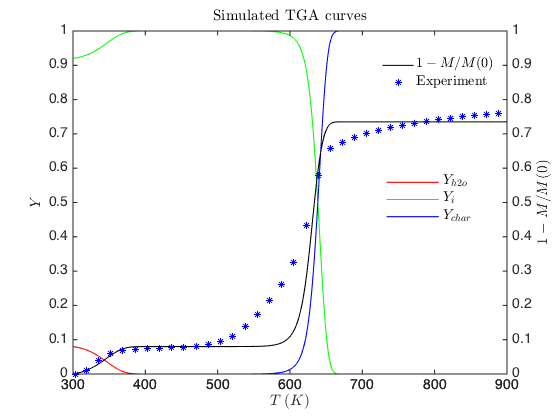
\includegraphics[scale=0.5]{tga.png}
\caption{Comparison of simulated and experimental TGA curves.}
\label{fig:simulatedTGA}
\end{figure}

\clearpage
\newpage

To check sensitivity to the various input parameters, the activation energies and prefactors of moisture and pyrolysis are individually and systematically between $\pm 10\%$ of their measured values. 

All results are plotted in figure \ref{fig:sens}.
Colour key: red prefactor moisture, green prefactor pyrolysis, blue activation energy moisture, black activation energy pyrolysis. 
The red, blue, and black lines are virtually indistinguishable 
Visual inspection of this plot indicates that the most significant parameter is the prefactor of pyrolysis. 
This is perhaps simply because has it the biggest value and therefore the largest absolute variation within this test. 

\begin{figure}
\centering
  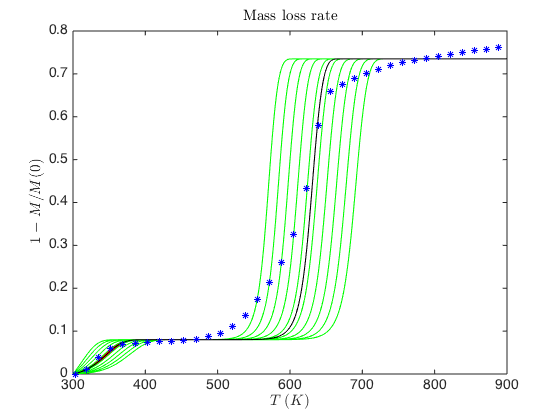
\includegraphics[scale=0.5]{sens.png}
\caption{Sensitivity to various parameters, see text for the explanation. Blue stars: experimental data.}
\label{fig:sens}
\end{figure}

\clearpage
\newpage
It is feasible to consider a simplified linear model. 
Here, oxygen mass and the change in the size and density of the fuel is assumed to be zero. 
The new system of ODEs is then
\begin{align}
\dot{\omega}_{pyr}&=\frac{1}{dT/dt}(H(T-T_0)-H(T-T_1))\frac{C_p}{\delta h_{pyr}}\frac{T-T_0}{T_1-T_0}\,,\\
\frac{d}{dT} Y_{H2O} &=\frac{1}{dT/dt}\frac{k_{H2O}}{\sqrt{T_s}} Y_{H2O} \exp(-E_{H2O}/(RT_s)) \,,\\
\frac{d}{dT}Y_i&=-\dot{\omega}_{pyr}\,,\\
\frac{d}{dT}Y_{char}&=(\nu_{char}-\nu_{soot})\dot{\omega}_{pyr}\,,
\end{align}

The new parameters $\frac{C_p}{\delta h_{pyr}}$ can be estimated (guessed) by fitting the numerical mass loss curve to the data in the specified pyrolysis range. 
Therefore this model is actually all numerical, the interpretation of the parameter as the ratio of specific heat capacity and heat of pyrolysis is not checked. 
It is therefore unknown how this parameter depends on heating rate and material. 
Because the fit is constructed the simulation matches the data almost exactly in the specified range. 
The values used in this simulation are $T_0=480$ K, $T_1=660$ K, and $C_p (T_1-T_0)/\delta h=2.4\times 10^{-4}$. 
All other parameters are the same as the previous simulation.
This model does not capture the degradation of the solid at high temperatures.
The results are shown in figure \ref{fig:simulatedTGAlinear}.
\begin{figure}[h!b]
\centering
  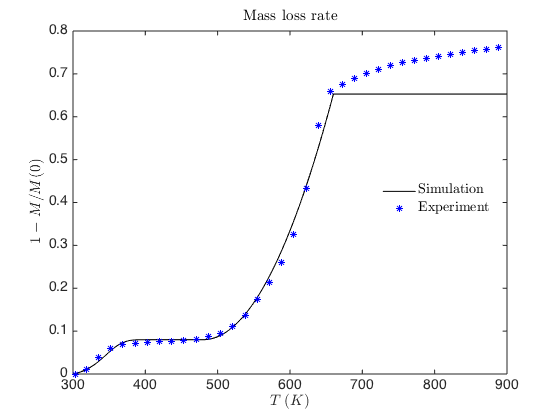
\includegraphics[scale=0.5]{tgaLinear.png}
\caption{Comparison of simulated and experimental TGA curves with the linear model. While the fit is good, the parameters do not necessarily have a physical meaning.}
\label{fig:simulatedTGAlinear}
\end{figure}

We attempt a systematic fit to the data by selecting an initial grid of $T_0$ and $T_1$ and then performing a least squares fit between the mass loss data and a pure quadratic (ie no linear nor constant terms). 
The ODE system is integrated and the choice of parameters which minimises the $L_2$ norm between the experimental data and the simulation is output.
The results are shown in figure \ref{fig:simulatedTGAfitted}.
Because of the method used to force the fit in this case, the overall mass loss result is an improvement over the simple linear model previously examined. 
The reason for poor agreement at higher temperatures is because there are reactions (of some kind) occurring during the experiment that are not modelled. 
This implies that perhaps taken the best fit between model and experiment over the whole mass-loss curve is not appropriate. 
The parameters for the best fit are the rate parameter $C_p(T_1-T_0)/\delta h=2.6899\times 10^{-5}$, $T_0=485$, and $T_1=670$. 
It must be stressed that these parameters have no physical meaning because they are simply from a numerical fit. 
Furthermore, by comparing these values to what was found manually there are large variations in the values of the parameters. 
\begin{figure}[h!b]
\centering
  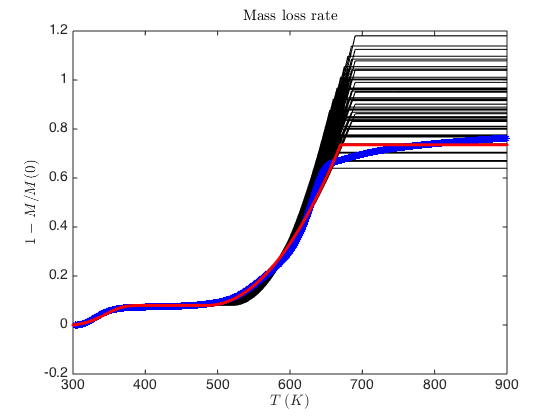
\includegraphics[scale=0.5]{tgaLinearFitted.png}
\caption{Comparison of simulated and experimental TGA curves with the linear model. The parameters were found by a simplistic optimisation scheme. While the fit is good, the parameters do not necessarily have a physical meaning. Blue: experiment, black: all trial solutions, red: best fit solution.}
\label{fig:simulatedTGAfitted}
\end{figure}

\end{document}
